\begin{figure*}[!thb]
  \centering
  \subfigure[Design Debt]{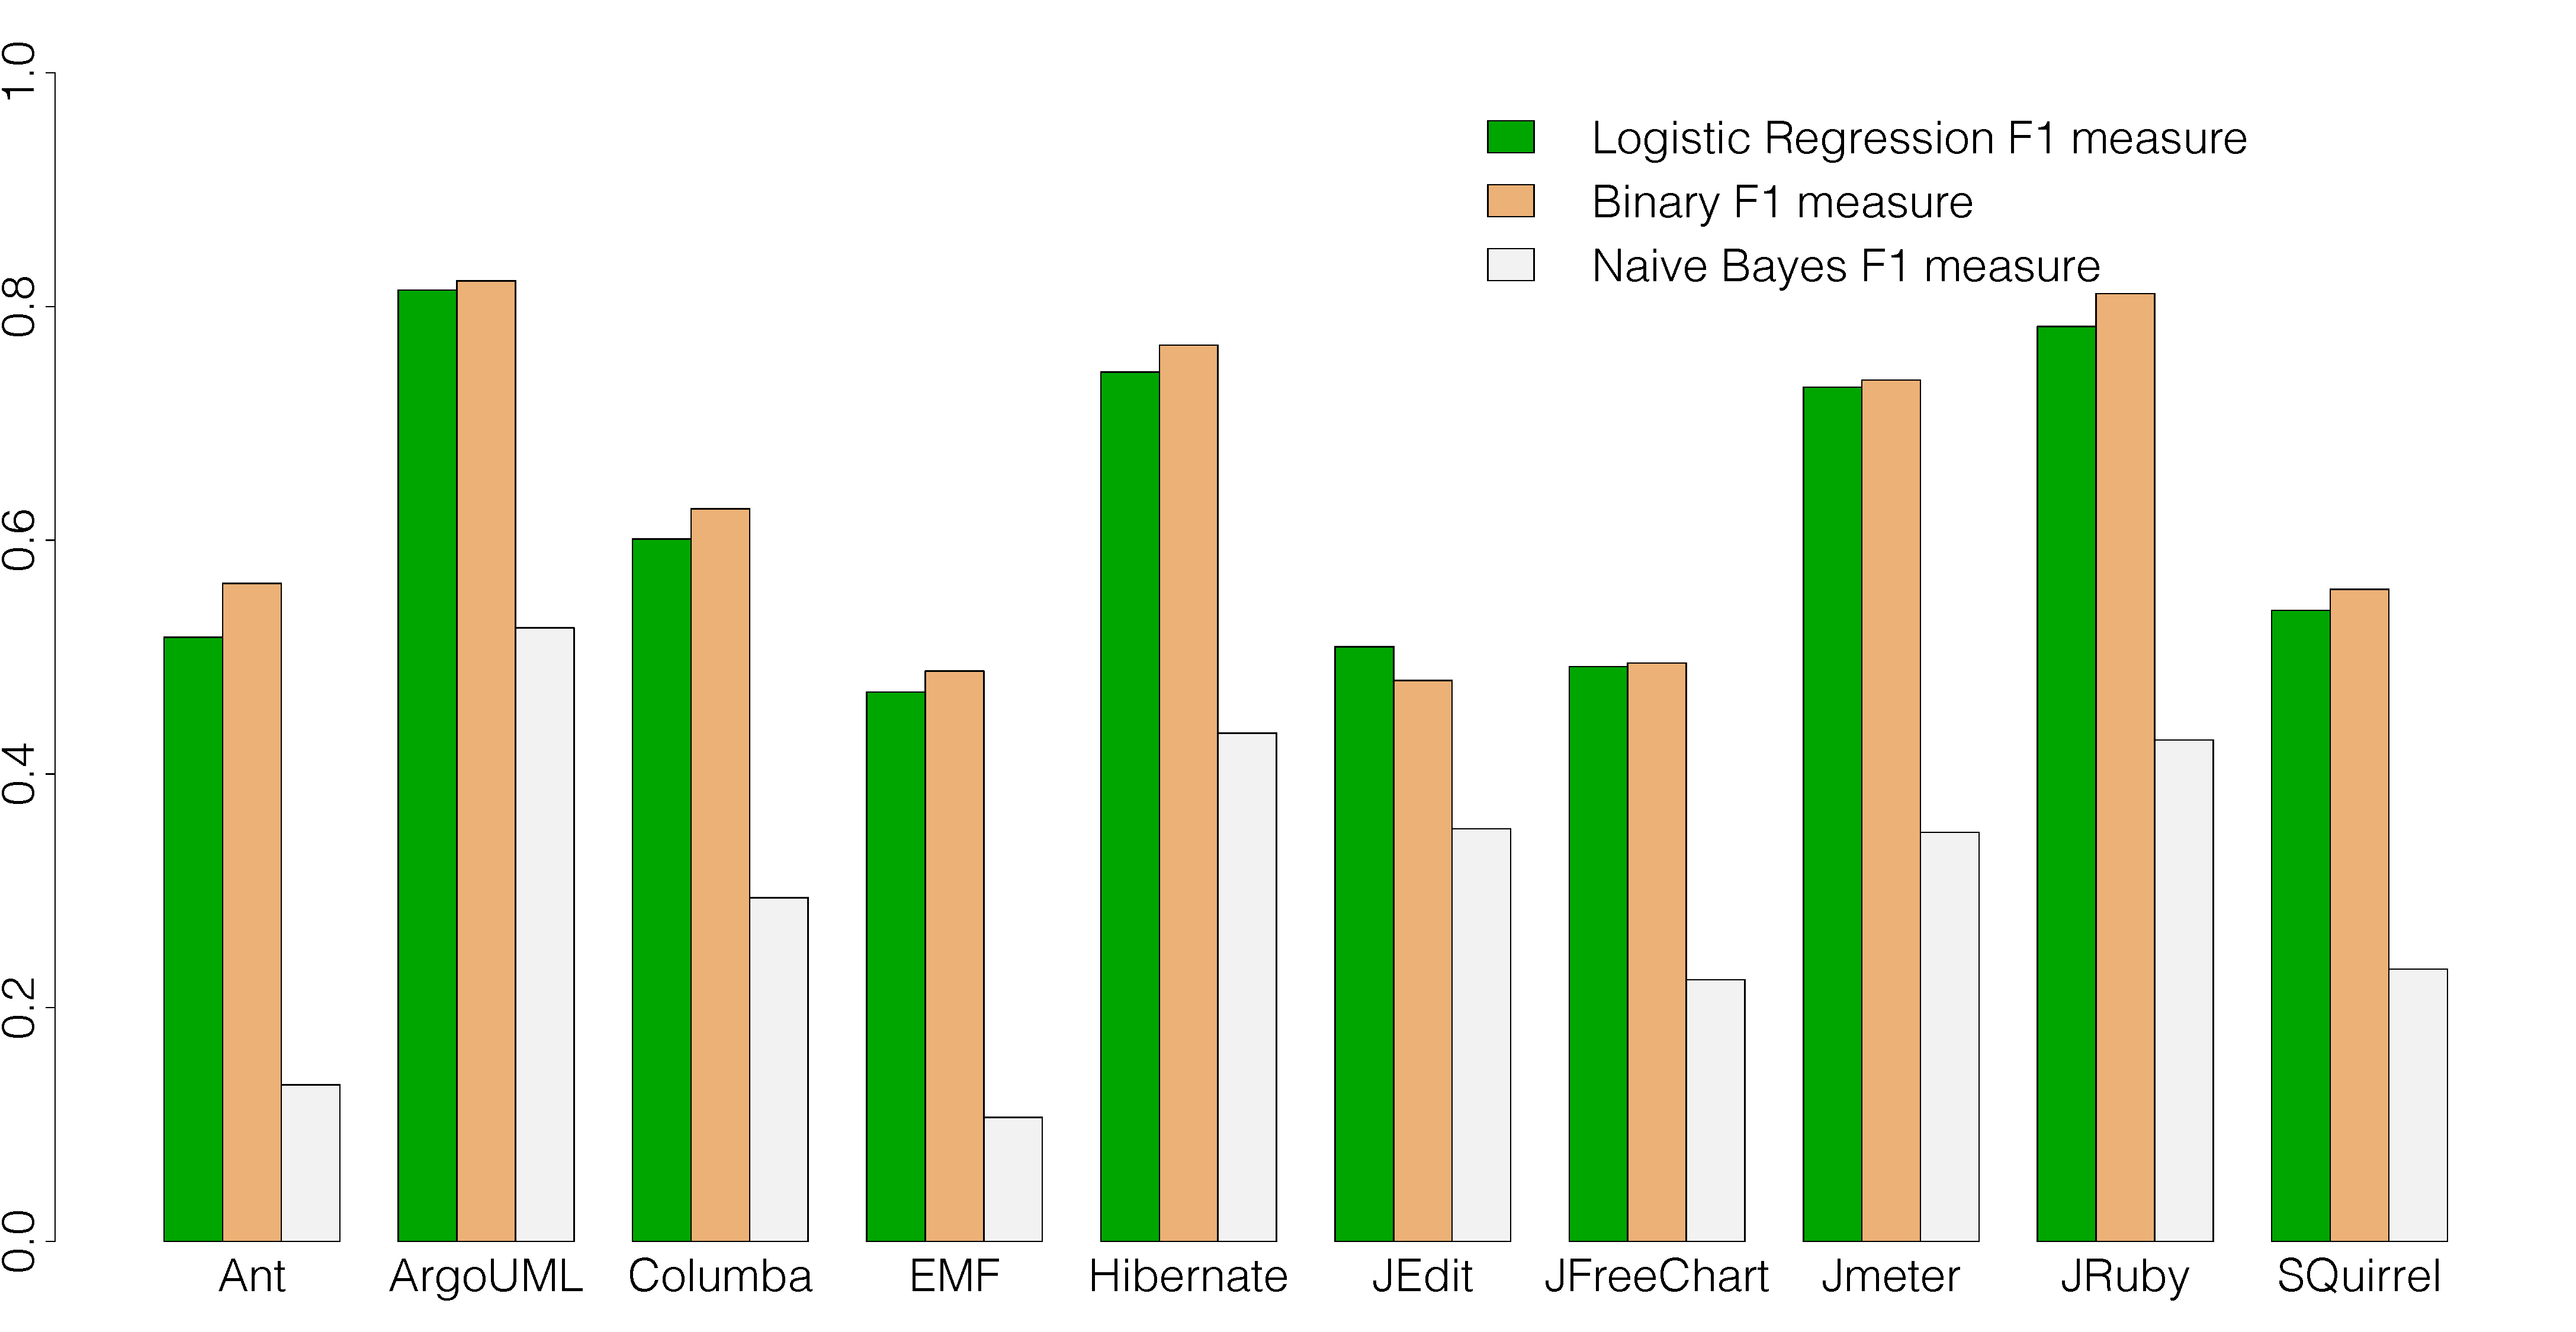
\includegraphics[width=0.48\textwidth]{figures/classifier_algorithms_comparison_design.pdf}
  \label{fig:algorithms_comparison_design}}
  \subfigure[Requirement Debt]{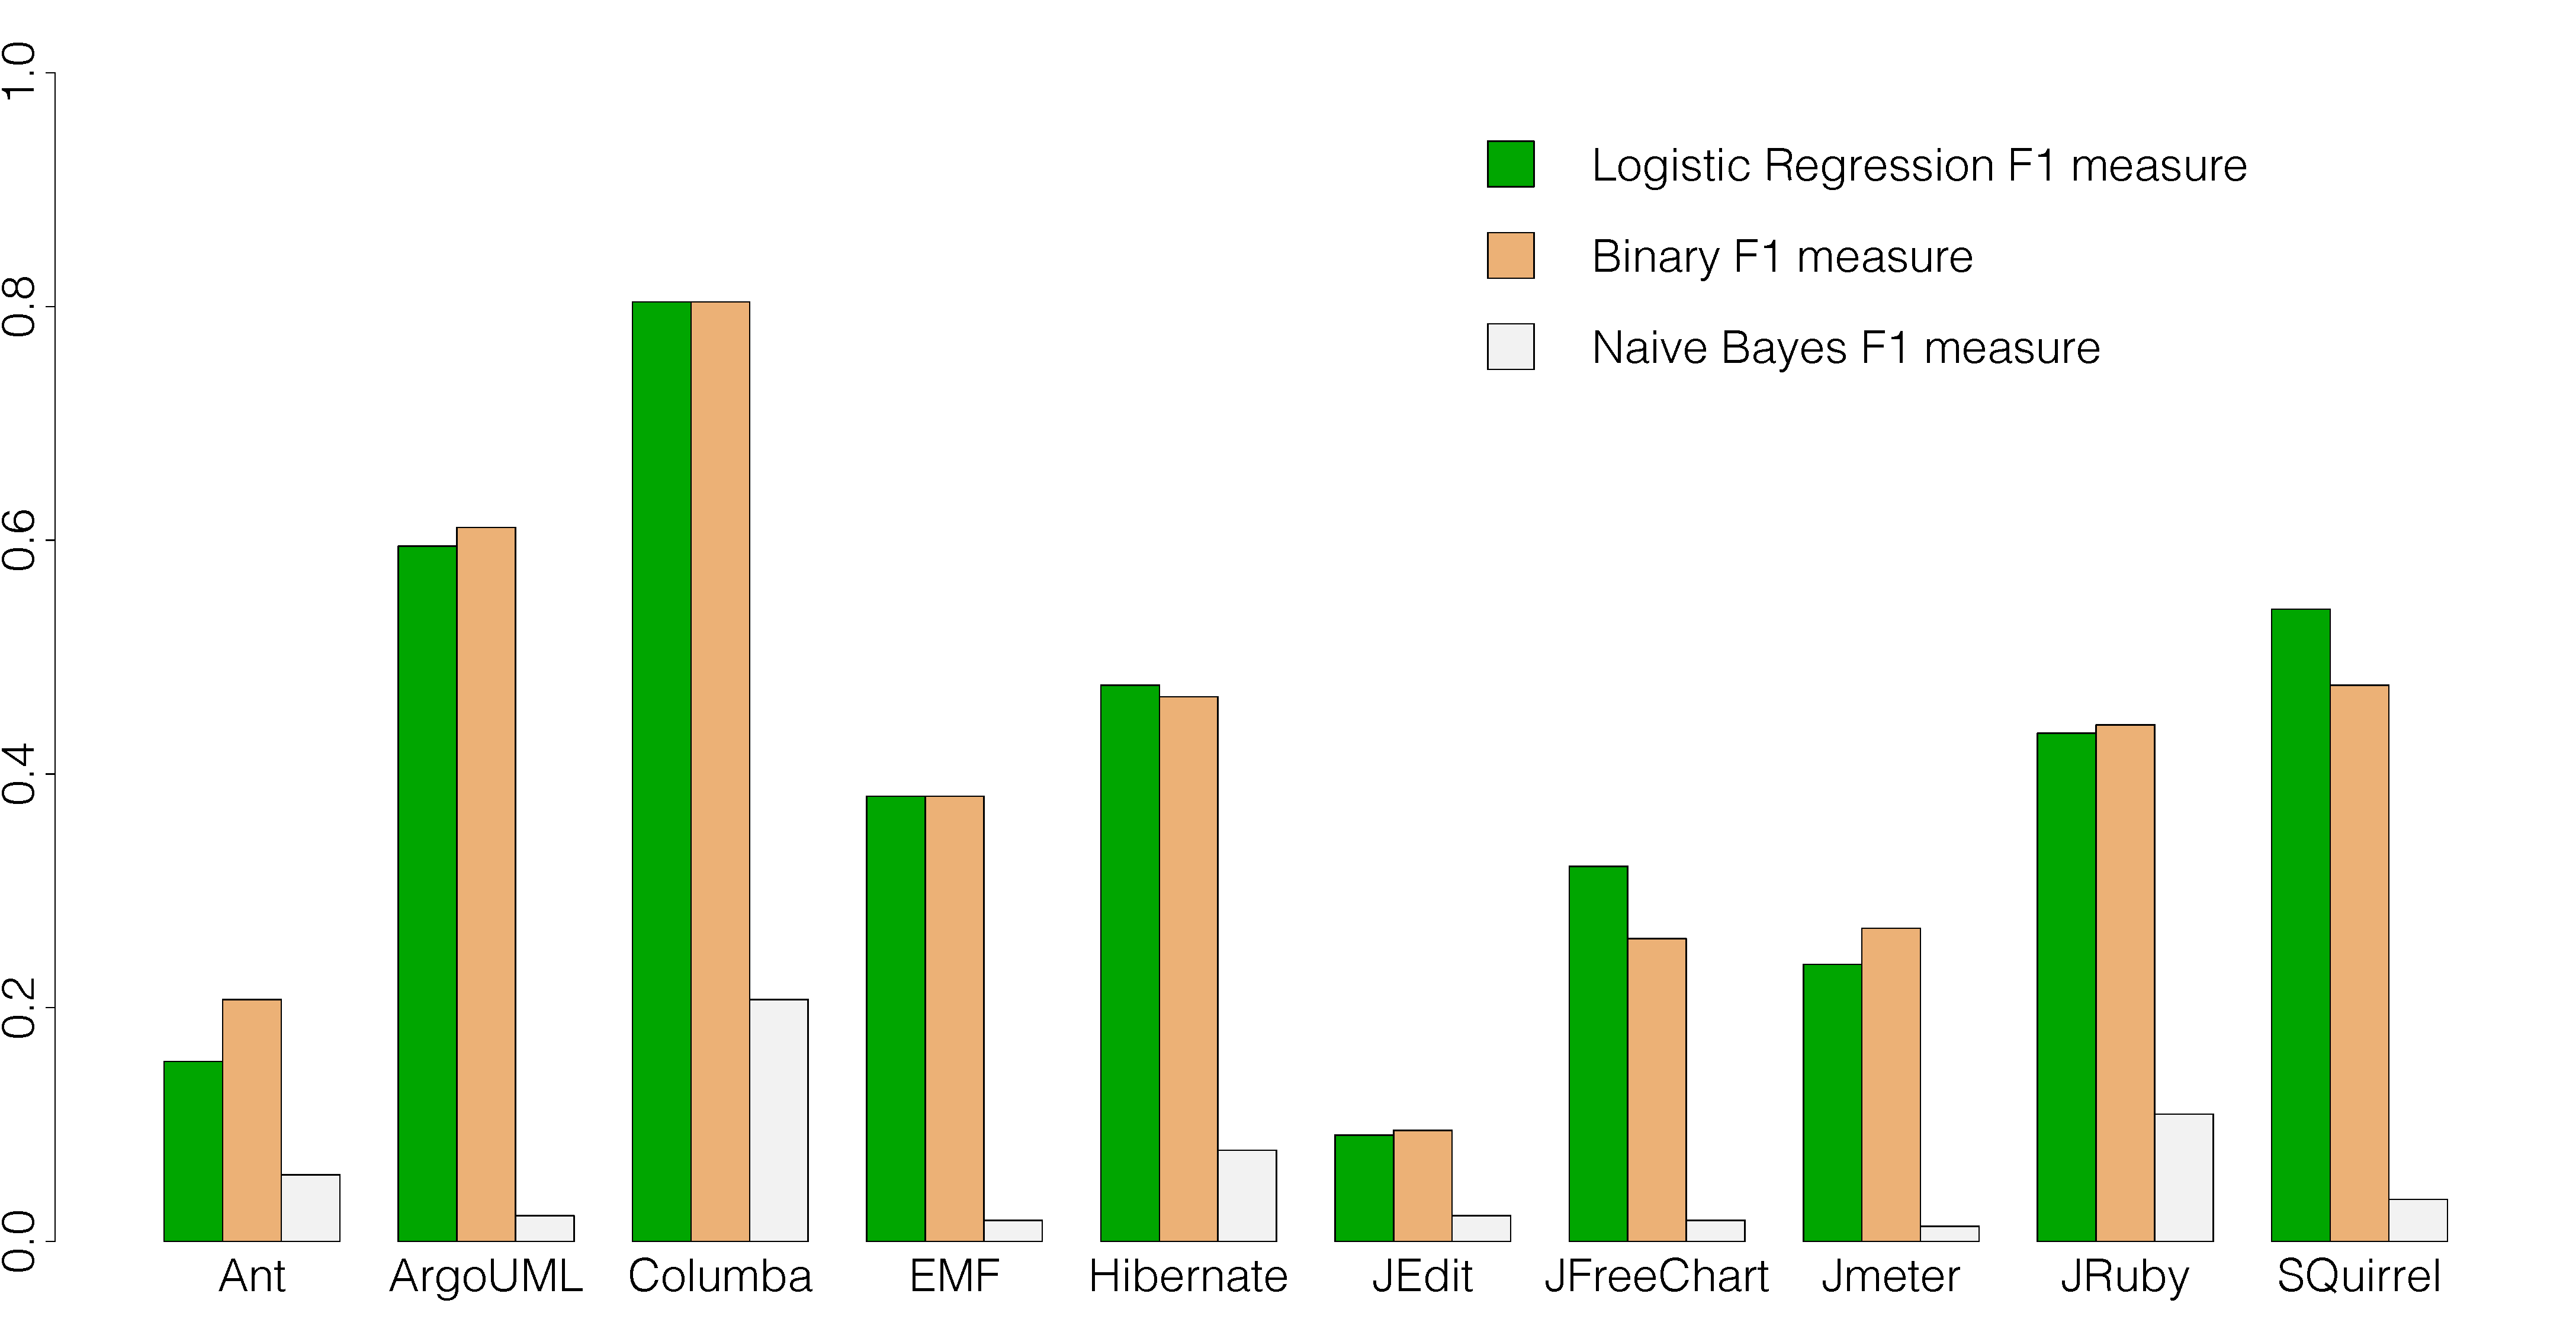
\includegraphics[width=0.48\textwidth]{figures/classifier_algorithms_comparison_requirement.pdf}
  \label{fig:algorithms_comparison_requirement}}
  \caption{Classification algorithms performance comparison}
  \label{fig:algorithms_comparison}
\end{figure*}

In this paper we propose an approach to identify \SATD comments using the Stanford Classifier. This tool, once trained correctly, can automatically classify natural language text. We create a training dataset of \SATD comments and analyzed the classification performance across ten open source projects. In RQ1, we show that our approach can outperform the current state-of-the-art in 10 out of 10 projects while identifying design and requirement debt. However, is not clear the reason why our approach was not equally effective across all projects. For example, JEdit has the worst F1 measure of all projects while classifying requirement \SATD.

By investigating JEdit comments, we notice two main reasons 1) the project has 10,322 comments. Of those only 14 are requirement \SATD. The data distribution represents a challenge to the classification. Even though the dataset is very unbalanced our precision was of 0.125 which compared with the random classifier baseline precision of 0.001 shows that our approach is still more useful. 2) Most requirement \SATD comments in this project are in the middle of long comments. Since our approach create a high number of prediction features for \SATD comments and also for without technical debt comments, long comments have more chances to match a higher number of without technical debt features. Therefore, long comments can generate `noise' that hinders the classification performance. One possible way to reduce this effect is through the addition of more similar data, as the addition of more similar data can change the prediction features generated by the classifier. 

Intuitively we know that each project has its own particularities, and that each group of developers, must often, create a unique way to communicate their concerns with each other. This unique trait of source code comments is inherited from the natural language itself and renders the fully automated prediction of every single \SATD very unlikely. Even when analyzing a old aged project, changes in the context of the application and turnover of developers can reflect changes in the way that source code comments are written. We can notice the impact of these particularities on the detailed performance analysis conducted in RQ3, where we can notice that the addition of more comments can eventually decrease the F1 measure performance.

For a great portion of \SATD comments there are common traits. Words as `workaround', `hack' are commonly imbued with criticism and the developers sense that this is not the appropriate solution for the problem in hand. However, relying just in these words for the identification of \SATD is not good enough as shown in Figures \ref{fig:f1_measure_comparison_design_debt} and \ref{fig:f1_measure_comparison_requirement_debt}. Therefore, NLP techniques, as proposed in our work, are needed in order to effectively identify \SATD comments.

In our work, all the classification done by the Stanford Classifier used a Logistic Regression classifier. However, would be interesting to see how other  algorithms perform when classifying our dataset. Then, we choose two other algorithms to execute the classification with: Naive Bayes generative classifier and Binary classifier.

As show in Figures \ref{fig:algorithms_comparison_design} and \ref{fig:algorithms_comparison_requirement}, while comparing the performance between the three different algorithms we find that the Naive Bayes has the worst average F1 measure: 0.308 and 0.058 for design and requirement \SATD respectively. The reason behind the low F1 measure average is that the Naive Bayes algorithm favors recall at the expense of precision. For example, while classifying design debt, the average recall was of 0.847 and precision 0.195.

The other two algorithms present more balanced results compared to Naive Bayes, and the difference in performance between them is not as accentuate. The Logistic Regression classifier achieved F1 measures of 0.620 and 0.403, while the Binary classifier F1 measures for design and requirement \SATD was 0.634 and 0.400 respectively. 

Although the Binary classification has a slightly better performance, for our research purpose, the Logistical Regression algorithm provide more insightful features as outcome. These features were analyzed and presented in RQ2. 